
\section{Study domain and earthquake data}

Thirty moderate-magnitude earthquakes ($3.5 > M_w > 5.5$), within period of 1998 to 2014, are considered for this study. The simulation domain, with a volume projection of \vdomain{180}{135}{62}{km}, covers the entire Los Angeles metropolitan area and most of the significant geologic structures around. Fig.~\ref{fig:region} shows the area of interest in which we labled the events with sequential letter code from A to Z and AA to AD and Table \ref{tab:events} provides their detailed information.The unprocessed recorded data from Southern California Earthquake Data Center (SCEDC) and Center for Engineering Strong Motion Data (CESMD) are downloaded for each earthquake to take advantage of the numerous time series available from different data centers. We obtain records for more than 800 stations overall, which provide us with enough available stations, even after removing the common stations or unusable ones, to make the results of evaluation acceptable.
\begin{figure}
    \centering
    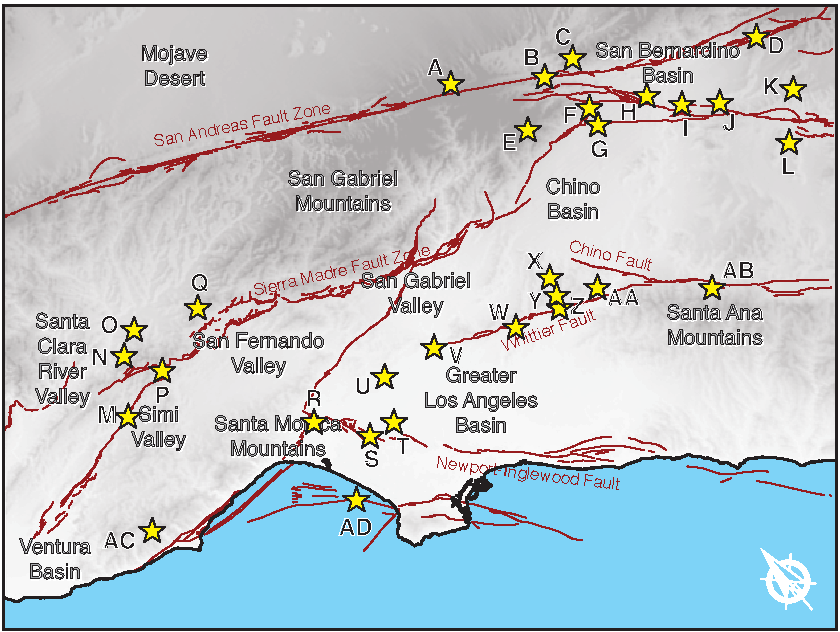
\includegraphics
 [width=\columnwidth]
     	{figures/pdf/figure-01}
    \caption{Major geologic structures in the region of interest including basins, valleys and mountains, along with the main quaternary faults.}
    \label{fig:region}
\end{figure}


\begin{table}
	\centering\small

	\caption{Information for 30 events including their ID \citet{SCEC}, magnitude and final number of stations.}
	\begin{tabular}{|c c c c || c c c c}
	
	\hline

	  	Code								& 
	  	Event ID							& 
	  	\eqmag{w}							&
	  	Num.								&
	  	Code								& 
	  	Event ID							& 
	  	\eqmag{w}							&
	  	Num.								\\
	\hline																																
		A			&	 9064568	&	4.40	&	17&  P&	14312160	&	4.66	&	109	\\ % A 

		B				&	10972299	&	3.79	&	52&	Q&	15237281	&	3.86	&	120\\ % R
		C				&	14494128	&	3.72	&	77&	R&	 9703873	&	4.24	&	130\\ % Z
		D					&	14155260	&	4.88	& 172&	S&	10410337	&	4.70	&	213\\ % V
																					
		E		&	10216101	&	3.60	&	55&	T&	 9716853	&	3.98	&	55\\ % J
																					
		F				&	13692644	&	3.74	&	55&	U&	 9093975	&	3.77	&	25\\ % S
		G				&	14116972	&	4.42	&	83&	V&	14601172	&	4.44	&	180\\ % U
		H			&	10370141	&	4.45	&	159 &	W&	15481673	&	5.10	&	311\\ % L
		I			&	 9140050	&	4.37	&	38&	X&	14383980	&	5.39	&	335\\ % D
		J					&	10541957	& 4.10&	97&	Y&	 9818433	&	4.75	&	67\\ % Q
		K				&	10530013	&	4.28	& 76	& Z&	10399889	&	3.98	&	91\\ % P
		L				&	14239184	&	3.90	&	66&	AA&	 9644101	&	3.64	&	53\\ % W
																					
		M				&	14000376	&	3.59	&	54&	AB&	10275733	&	4.73	&	116\\ % T
		N			&	 9753489	&	3.90	&	52&	AC&	10403777	&	4.42	&	94\\ % H
		O			&	 9096972	&	3.98	&	26&	AD&	14738436	&	3.69	&	93\\ % C
		\hline
																				
	\end{tabular}
	\label{tab:events}
\end{table}



